% use tuhh template
% can be found here: https://www.tuhh.de/

\documentclass[10pt]{article}
\usepackage[utf8]{inputenc}
\usepackage{graphicx}
\usepackage{amsmath}
\usepackage{amssymb}
\usepackage{algorithm}
\usepackage{algorithmicx}
\usepackage{algpseudocode}
\usepackage{hyperref}


\date{February 2023}
% create title
\title{PACE Challenge 2023 - Twin-width}
\author{
    Constantin Duske, Karl Henning, Johann Strunck\\
    email: \texttt{\{constantin.duske, karl.henning, johann.strunck\}@tuhh.de}
}

\begin{document}

\maketitle
\section{Abstract}



\section{Introduction}
%unnötige introduction .. \\

In the course of the seminar Algorithm Engineering we participate in the \href{https://pacechallenge.org/2023/}{PACE Challenge 2023}. This years
Challenge is about twin-width, a graph parameter that measures the distance of a graph to
a co-graph. Introduced in 2020 The parameter did lead to many theoretical results but as
of now its not real practical tested. The goal of this paper is to implement and test it to bridge
the gap between theory and practice.\\ The twin-width algorithm is an new approach to
solve graph theory problems that are commonly solved by the tree-width algorithm. The
starting point of our paper will be a short summary of the algorithm. Afterwards we will
introduce a way to implement it in C++ and present how it performs on a test set of graphs.
%Beschreibung...

\section{Twin Width}
The twin-width of a graph is an indicator for its complexity and studies how efficient
different algorithms will perform.

Basically it's a non-negative integer measuring a graphs distance to being a Cograph. A
Cograph is described by the following properties:

\begin{enumerate}
    \item K1 is a Cograph.
    \item If G is a Cograph the complement of G is also a Cograph.
    \item If G and U are Cographs their disjoint union is also a Cograph.
\end{enumerate}

This implies that you can find two twins in every Cograph, that you can contract together
and iterate the process until you have only a singleton left.

Now the idea is that a graph has bounded twin-width if we can contract it to a singleton
by contracting near-twins together (two vertices whose neighborhoods differ only on a
bounded number of elements). We actually track the errors and call the edges we need to
add "red edges".

A graph has now twin-width d if we can bound the degree in red edges by the treshhold d.
Because Cographs don't produce errors they always have twin-width 0. \\
%Add grapic example

graphs that can be reduced to a single vertex by a process of repeatedly finding any two
twin vertices and merging them into a single vertex. The definition of twin-width mimics
this reduction process. there are false and true twins.

true twins have the same set of edges A = B false twins have a similar set of edges the
edges that differ will be marked red {A / B \& B/A} == red

the twin width is the variable that sets the maximum of red edges that appear by a
reduction of a graph G. This variable can be used to upper-bound the complexity for
certain algorithms from NP-Complexity to Polynomial Complexity. citations:
\cite{bonnet2021twini} \cite{bonnet2021twinii}.




\section{Algorithm}

% requires package algorithmicx
\begin{algorithm}[H]
    \caption{Greedy Algorithm}
    \label{alg:greedy}
    \begin{algorithmic}[1]
        \State \textbf{Input:} Graph G
        \State \textbf{Output:} Upper bound for the twin-width of G
        \State \textbf{Initialize:} $minMerges \gets \emptyset$
        \For{each vertex $v$ in $G$}
        \State $minMerges[v] \gets getOptimalMerge(v)$
        \EndFor
        \For{each iteration}
        \State $optimalMerge \gets (redDeg = \infty, target = 0, del = 0)$
        \For{each vertex $v$ in $G$}
        \If{$v$ is deleted}
        \State \textbf{continue}
        \EndIf
        \State $merge \gets minMerges[v]$
        \If{$v$ has no neighbours}
        \State delete $v$
        \State \textbf{break}
        \EndIf
        \If{$merge.redDeg < optimalMerge.redDeg$}
        \State $optimalMerge \gets merge$
        \EndIf
        \If{$optimalMerge.redDeg == 0$}
        \State \textbf{break}
        \EndIf
        \EndFor
        \If{$optimalMerge.redDeg == \infty$}
        \State \textbf{continue}
        \EndIf
        \State perform merge
        \State $minMerges[optimalMerge.del] \gets (redDeg = \infty)$
        \State update $target$ and its first, second and third degree neighbours
        \EndFor
    \end{algorithmic}
\end{algorithm}

\subsection{Greedy Algorithm}
The greedy algorithm is a simple algorithm that iteratively finds the most optimal next
merge. The procedure begins by finding the most optimal next merge by trying out all
possible merges and calculating the maximal number of red edges that emerge from each
vertex. To do this, we have written code that avoids creating copies of the "original"
graph. After an optimal merge is found, we perform the merge and repeat the process until
only a single vertex remains.

\subsection{Heuristic}
To further optimize our algorithm, we added a heuristic which only considers merges of
first and second-degree neighbors. This heuristic is always optimal because vertecies of
degree greater than two will always result in a higher number of red edges.

\subsection{Caching}
To further optimize our algorithm, we added a caching mechanism which stores for every
vertex its optimal merge partner and the resulting maximal number of red edges in which
the merge would result. This allows us to avoid recalculating the optimal merge for every
vertex. This is especially useful for large graphs.

\section{Example}
In the following we will show our algorithm in action on a small graph. The vertecies are
labeled according to the following schema (index, optimal merge partner, resulting
maximal number of red edges after merge). The optimal merge partner is the index of the
vertex that should be merged with the current vertex. The maximal number of red edges is
the number of red edges that would result from the merge. The colors of the edges
indicate the following:
\begin{itemize}
    \item green: default color
    \item orange: optimal merge partner updated. Old optimal merge partner got deleted
    \item red: optimal merge partner updated. Old optimal merge partner did not got deleted
    \item blue: optimal merge partner did not get updated. Only the maximal number of red edges
          after merge got updated
\end{itemize}

% Why did we introdruced the colors? 
% We should explain the colors in the example

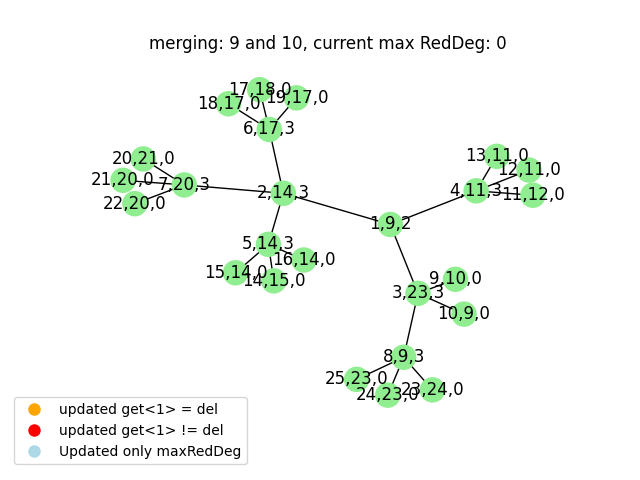
\includegraphics[width=0.5\textwidth]{images/merge0.png}
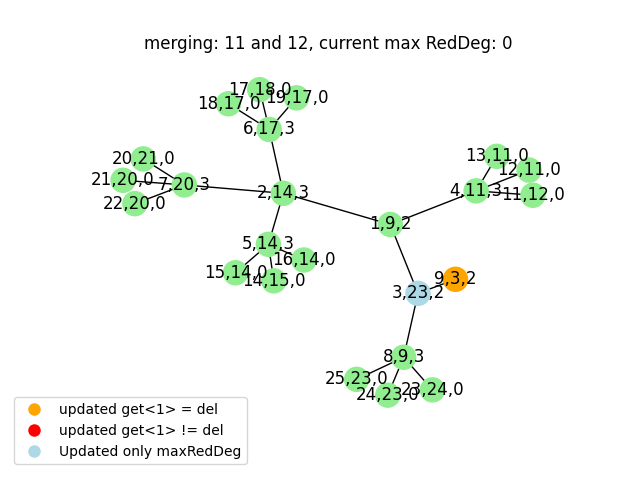
\includegraphics[width=0.5\textwidth]{images/merge1.png}
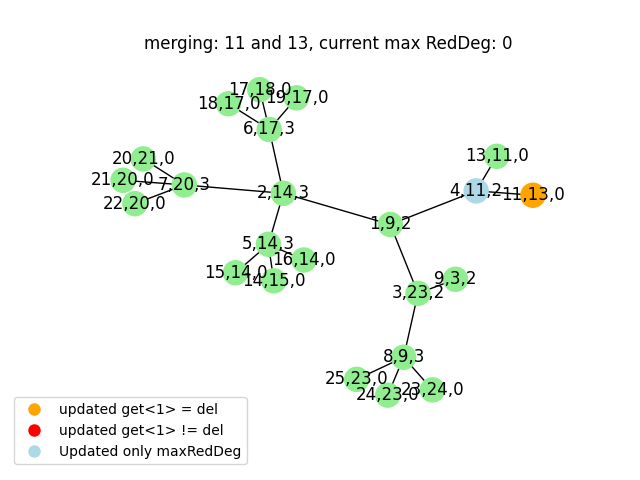
\includegraphics[width=0.5\textwidth]{images/merge2.png}
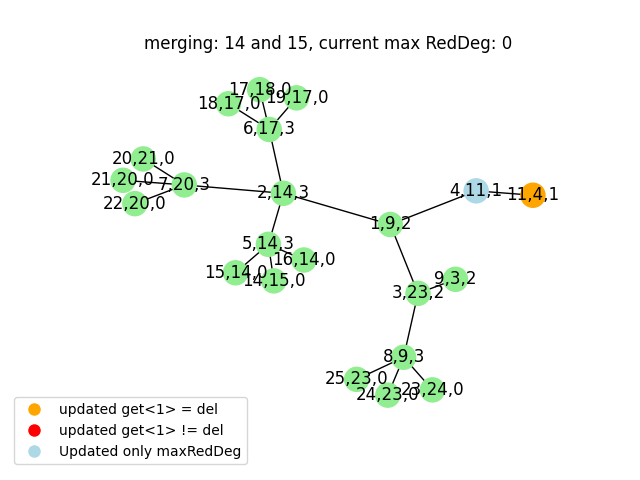
\includegraphics[width=0.5\textwidth]{images/merge3.png}
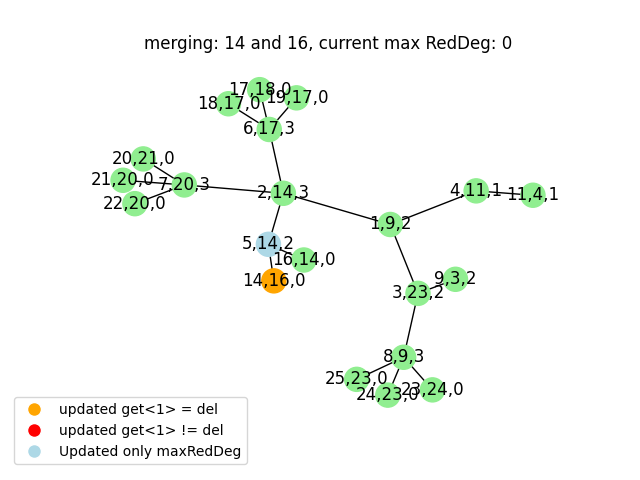
\includegraphics[width=0.5\textwidth]{images/merge4.png}
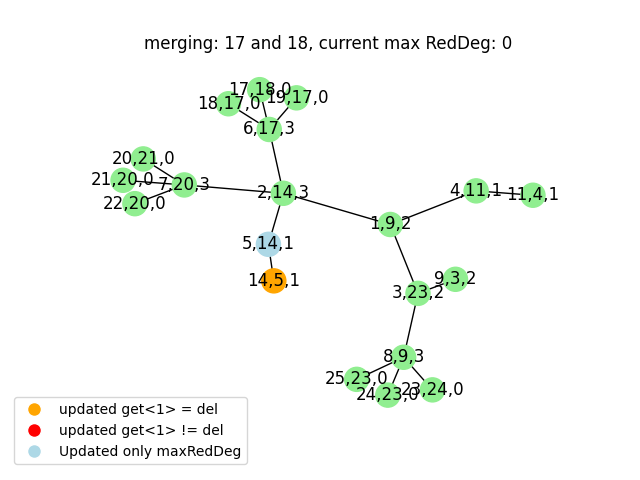
\includegraphics[width=0.5\textwidth]{images/merge5.png}
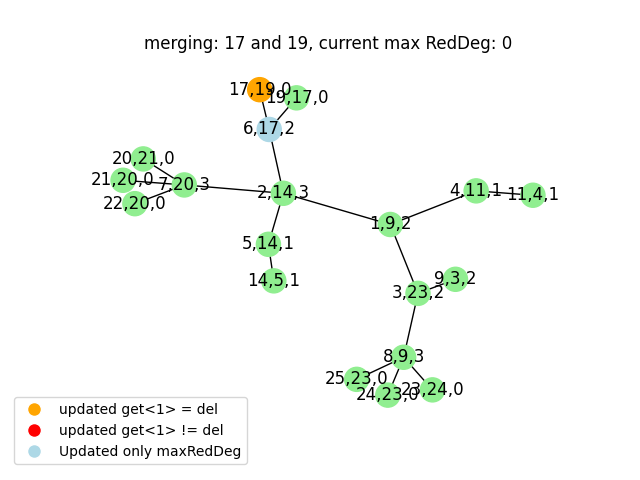
\includegraphics[width=0.5\textwidth]{images/merge6.png}
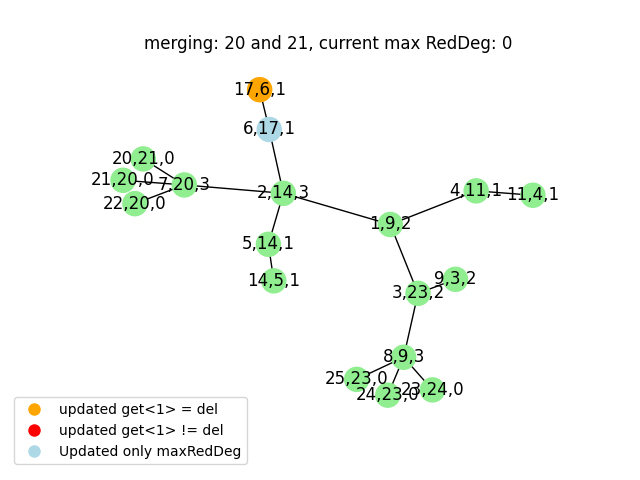
\includegraphics[width=0.5\textwidth]{images/merge7.png}
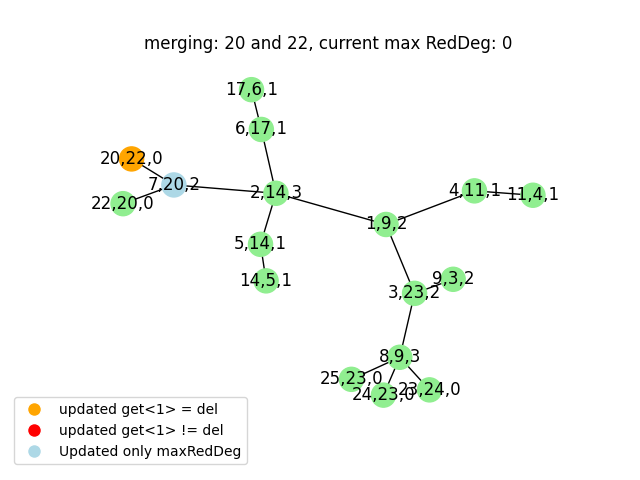
\includegraphics[width=0.5\textwidth]{images/merge8.png}
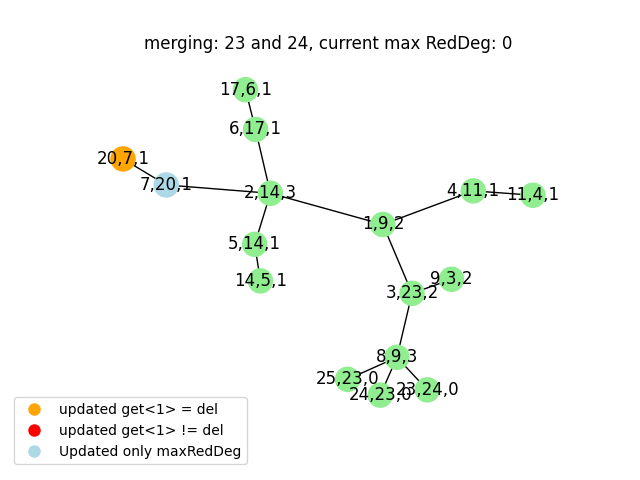
\includegraphics[width=0.5\textwidth]{images/merge9.png}
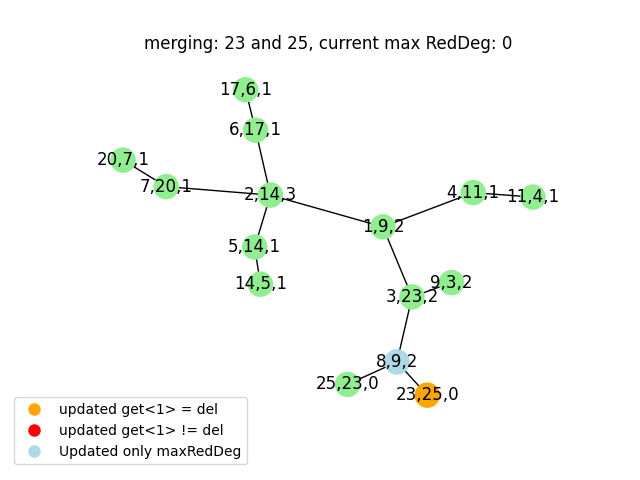
\includegraphics[width=0.5\textwidth]{images/merge10.png}
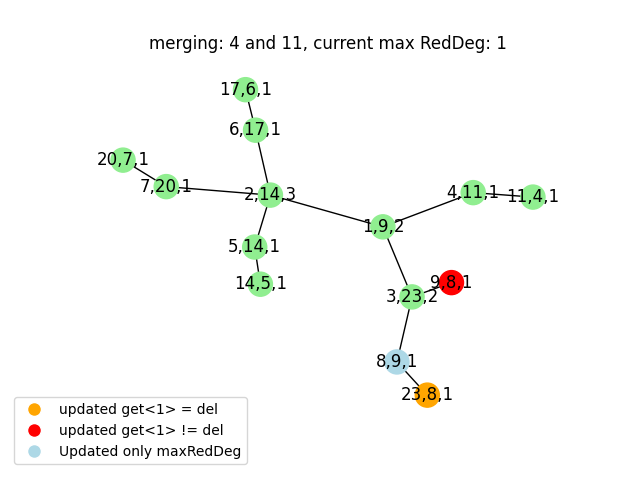
\includegraphics[width=0.5\textwidth]{images/merge11.png}
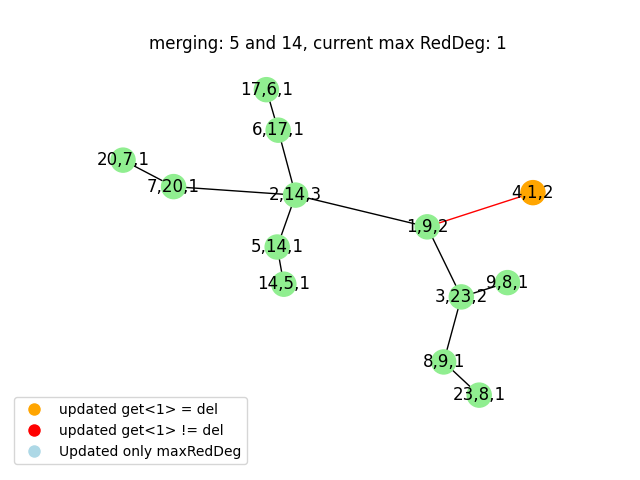
\includegraphics[width=0.5\textwidth]{images/merge12.png}
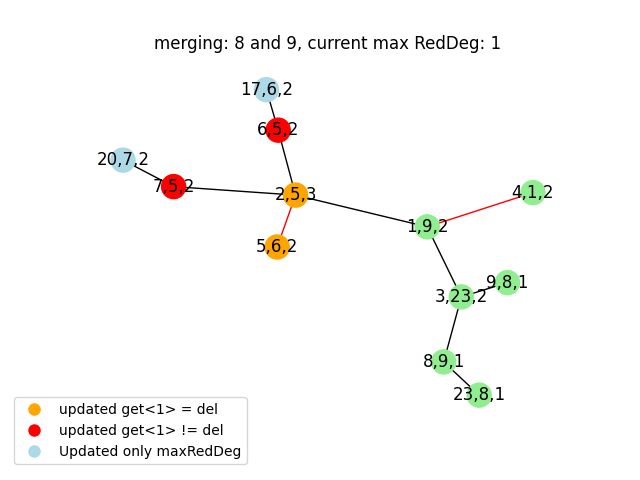
\includegraphics[width=0.5\textwidth]{images/merge13.png}
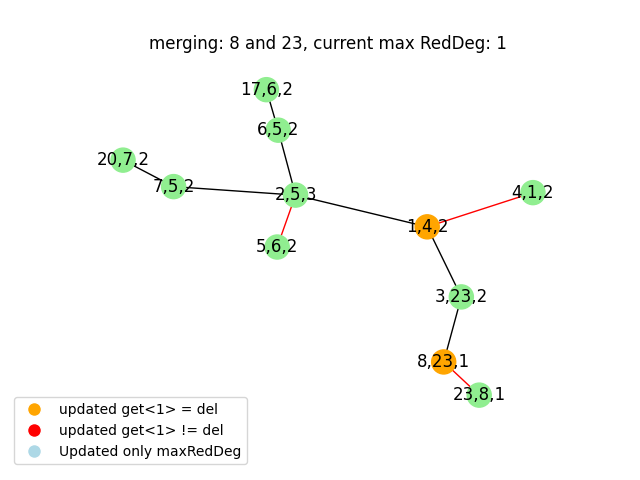
\includegraphics[width=0.5\textwidth]{images/merge14.png}
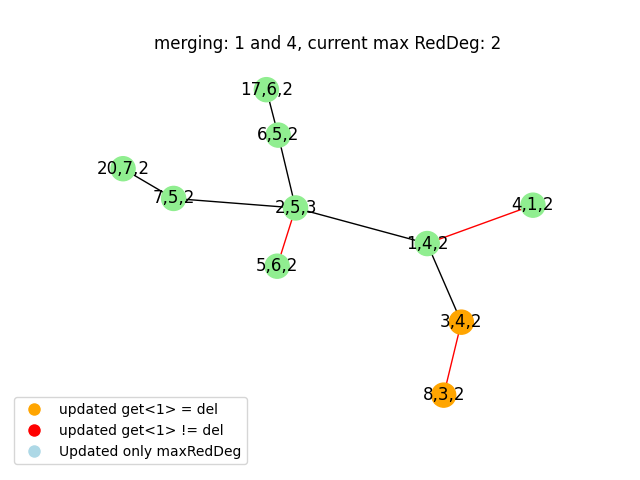
\includegraphics[width=0.5\textwidth]{images/merge15.png}
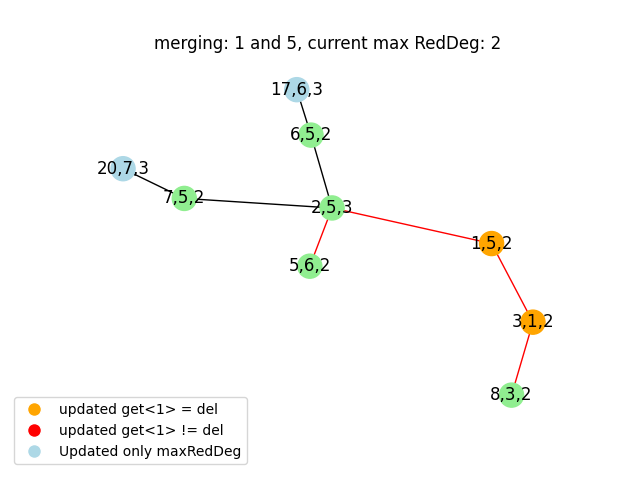
\includegraphics[width=0.5\textwidth]{images/merge16.png}
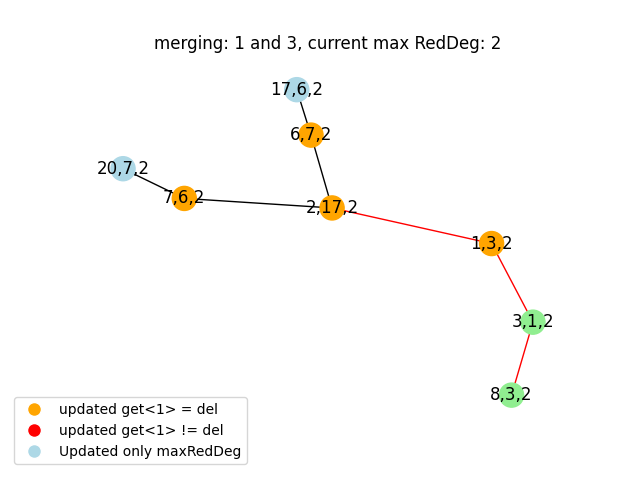
\includegraphics[width=0.5\textwidth]{images/merge17.png}
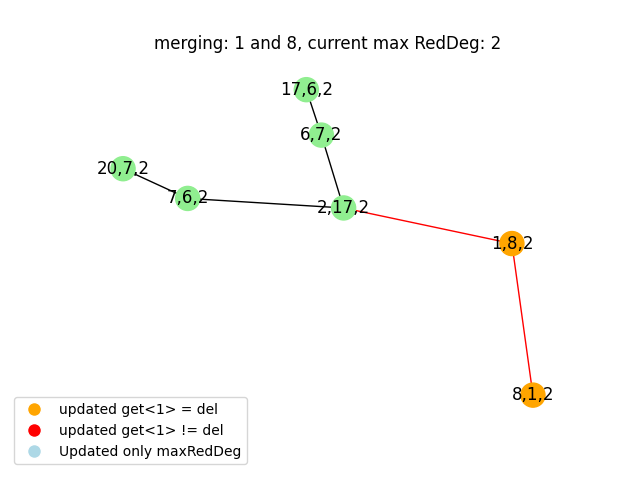
\includegraphics[width=0.5\textwidth]{images/merge18.png}
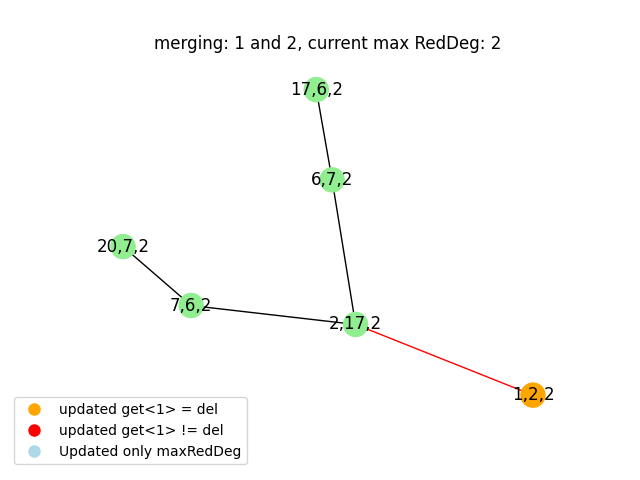
\includegraphics[width=0.5\textwidth]{images/merge19.png}
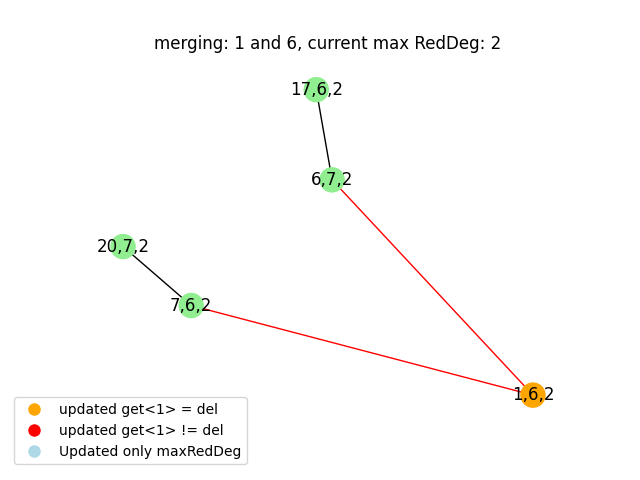
\includegraphics[width=0.5\textwidth]{images/merge20.png}
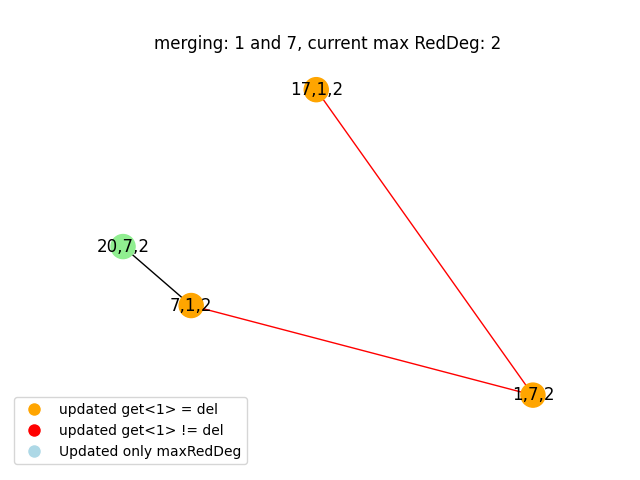
\includegraphics[width=0.5\textwidth]{images/merge21.png}
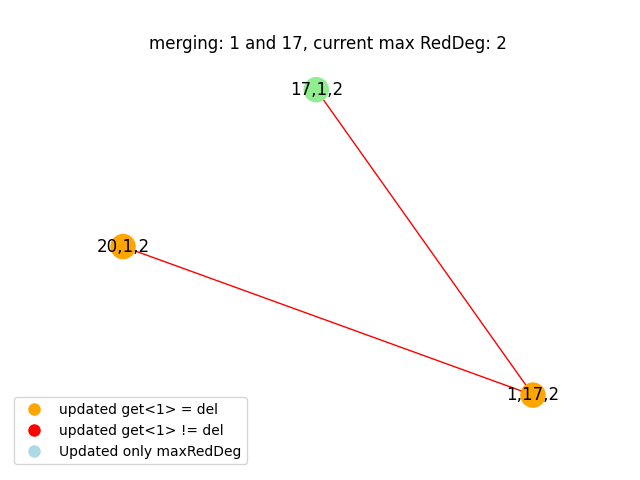
\includegraphics[width=0.5\textwidth]{images/merge22.png}
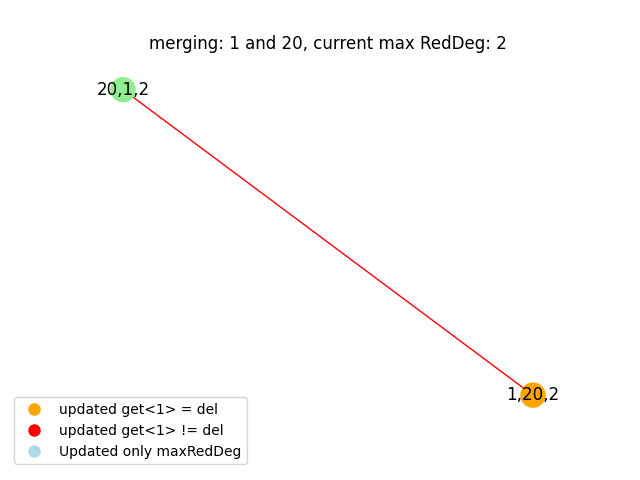
\includegraphics[width=0.5\textwidth]{images/merge23.png}
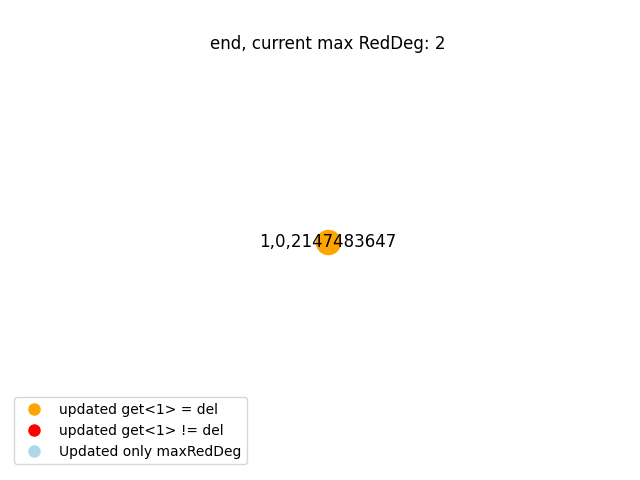
\includegraphics[width=0.5\textwidth]{images/merge24.png}

\section{Results}
We have tested our algorithm on a variety of graphs.

\section{Conclusion}

\bibliographystyle{ACM-Reference-Format}
\bibliography{bibliography}
% \citestyle{acmauthoryear}

\end{document}
